\documentclass[usenames,dvipsnames, aspectratio=169, 9pt]{beamer}
\beamertemplatenavigationsymbolsempty
\setbeamertemplate{footline}[frame number]
\setbeamertemplate{section in toc}[sections numbered]
\usecolortheme[named=Plum]{structure}
\usefonttheme{serif}
\usepackage{amsmath, amsthm, amssymb, pgffor, multirow, booktabs, tabularx, multirow, graphicx, pgffor, arydshln}
\usepackage{booktabs}
\usepackage{kotex}
\usepackage{epstopdf}
\usepackage{grffile}


\author{Boyeon Kim}
\institute{Department of Mathematics, School of Mathematics and Computing \\ Mathematics \\ Yonsei University}
%\date{January 6, 2023}
\title{Reinforcement Learning Seminar}

\def\bs{\boldsymbol}
\usepackage{grffile}
\begin{document}

  \maketitle

\begin{frame}{SEIAR Optimal control}
    \begin{itemize}
        \item Previous experiments have shown that for one control, \\ we can find optimal control using reinforcement learning.
        \item By introducing a new problem that is one control, \\we will try to do optimal control in the following two ways.  
        \item Goal1 : DQN
        \item Goal2 : PPO
    \end{itemize}
\end{frame}


\begin{frame}\frametitle{Mathematical models}
    \begin{itemize}
        \item The influenza model : SEIAR model 
        \item J.Kim et.al.,\textit{Constrained optimal control applied to vaccination for influenza},2016
    \end{itemize}
    \begin{align*}
        S'(t) &= -\beta S(t) \Lambda(t) - \psi \nu(t) S(t)\\
        E'(t) &= \beta S(t) \Lambda(t) - \kappa E(t)\\
        I'(t) &= p\kappa E(t) - \alpha I(t) - \tau I(t) \\
        A'(t) &= (1-p)\kappa E(t) - \eta A(t) \\
        R'(t) &= f \alpha I(t) + \tau I(t) + \eta A(t) + \psi \nu(t) S(t)
   \end{align*}
with $\Lambda(t) = \epsilon E(t) + (1 - q) I(t) + \delta A(t)$ 
    
    \centering
    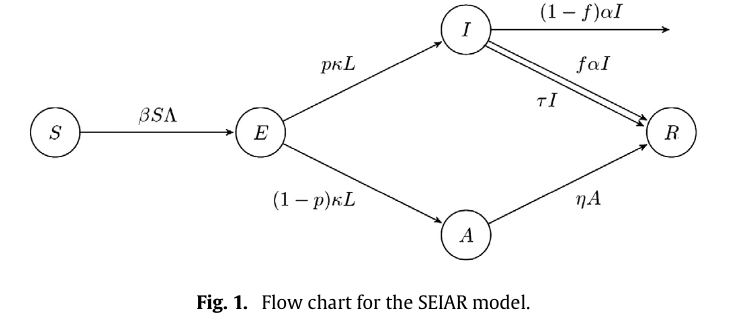
\includegraphics[width=8cm]{figures/model.png}
\end{frame}


\begin{frame}\frametitle{SEIAR model parameters}
\begin{table}[]
\begin{tabular}{lll}
\hline
Parameter & Description                                       & value        \\ \hline
$\epsilon$   & Infectivity reduction factor for the exposed      & 0            \\
$q$         & Contact reduction by isolation                    & 0.5          \\
$\delta$     & Infectivity reduction factor for the asymptomatic & 0.5          \\
$p$         & Fraction of developing symptoms                   & 0.667        \\
$\kappa$     & Transition rate for the exposed                   & 0.7143 / day \\
$f$         & Complement to fatality rate (1 - fatality rate)   & 0.999        \\
$\alpha$     & Recovery rate for the (symptomatic) infective     & 0.1667 /day  \\
$\eta$       & Recovery rate for the asymptomatic                & 0.1667 / day \\
$\tau$       & Antiviral treatment rate                          & 0 / day      \\
$\psi$       & Efficacy of vaccination                           & 70\%         \\ 
$\beta$    & Transmission rate                                 & 6.3346e-08           \\
$R_{0}$     & Basic Reproduction number                         & 1.9           \\\hline
\end{tabular}
\end{table}
\begin{itemize}
    \item $S0 = 5e07, \quad E0 = 0, \quad   I0 = 1,   \quad  A0 = 0,  \quad   R0 = 0$
\end{itemize}
\end{frame}


\begin{frame}\frametitle{Goal in paper}
\begin{itemize}
    \item The goal is to \textcolor{Plum}{\textbf{minimize the number of people who become infected}} at a \textbf{minimal efforts of vaccination}.
    \item The objective functional is given by
\end{itemize}
\begin{align*}
J(\nu) = \int_0^T P I(t) + Q \nu^2(t) dt\\
\end{align*}
with inequlity constraints
$0 \leq \nu(t) \leq 1$, \quad $\nu(t) S(t) \leq \nu_{max}$, \quad $z(t) = \int_0^T \nu(t) S(t) \leq \nu_{total}$\\
\begin{itemize}
    \item $\nu_{max}$ : The maximum daily vaccination
    \item $\nu_{total}$ : Vaccine coverage
    \item $z'(t) = \nu(t) S(t)$ \quad $z(0) = 0$ \quad $z(T) \leq \nu_{total}$ \quad $z'(t) \leq \nu_{max}$
\end{itemize}
\end{frame}

\begin{frame}\frametitle{penalty method}
\begin{itemize}
    \item \textcolor{Plum}{The constrained optimal control} $\rightarrow$ \textcolor{Plum}{into unconstrained optimization} problems.
    \item The objective penalty function
\end{itemize}
\begin{align*}
J_p(\nu) &= \int_0^T P I(t) + Q \nu^2(t) 
\\ &+ \mu_1 (\nu(t) S(t) - \nu_{max})^2 H_1 (\nu(t)S(t) - \nu_{max}) 
\\ &+ \mu_2 (z(t) - \nu_{total})^2 H_2 (z(t) - \nu_{total}) dt\\
\end{align*}
with Heaviside step function
\begin{align*}
H_1 (\nu(t)S(t) - \nu_{max}) &=
\begin{cases}
0 \quad\quad if \quad \nu(t)S(t) \leq \nu_{max} \\ 1 \quad\quad if \quad \nu(t)S(t) > \nu_{max} \\
\end{cases}
\\H_2(z(t) - \nu_{total}) &=
\begin{cases}
0 \quad\quad if \quad z(t) \leq \nu_{total} \\ 1 \quad\quad if \quad z(t) > \nu_{total} \\
\end{cases}
\end{align*}
with $z(t) = \int_0^T \nu(t) S(t) dt$
\begin{itemize} 
    \item $z'(t) = \nu(t)S(t)$ \quad $z(0) = 0$ \quad $0 \leq \nu(t) \leq 1$
\end{itemize}
\end{frame}

\begin{frame}
\centering
\textcolor{Plum}{\textbf{Reinforcement Learning}}
\end{frame}

\begin{frame}\frametitle{Set the environment for DQN}
\begin{itemize}
    \item $\nu_{max} = 5e05 (0.01 * S0) $
    \item $\nu_{total} = 5e06 (0.1 * S0)$
    \item Observation space : 5 (S, E, I, A, R)
    \item Action space : 2 (0 or 1)
    \item Action
    \begin{itemize}
            \item $\nu$ : the number of vaccinated people
            \item action = 0 $\rightarrow$ $\nu = 0$
            \item action = 1 $\rightarrow$ $\nu = \nu_{max}$
            \item $\nu$(ratio) = $\nu/\nu_{max}$
    \end{itemize}
    \item Reward design
        \begin{itemize}
            \item case1)
                \begin{itemize}
                    \item - I - $\nu$
                    \item if sum($\nu$) $> \nu_{total}$, penalty reward: - 10000
                \end{itemize}
            \item case2) Similar to the paper
                \begin{itemize}
                    \item -PI - Q$\nu(ratio)^2$  
                    \item if $\nu(ratio)*S(t) > \nu_{max}$,  penalty reward: -10000
                    \item if sum($\nu$) $> \nu_{total}$ , penalty reward: -10000
                    \item P, Q : proper weight
                \end{itemize}
        \end{itemize}
\end{itemize}
\end{frame}

\begin{frame}
\centering
\textcolor{Plum}{\textbf{Gaol1 : DQN}}
\end{frame}

\begin{frame}\frametitle{SELAR optimal: DQN}
\begin{itemize}
    \item Error
\end{itemize}
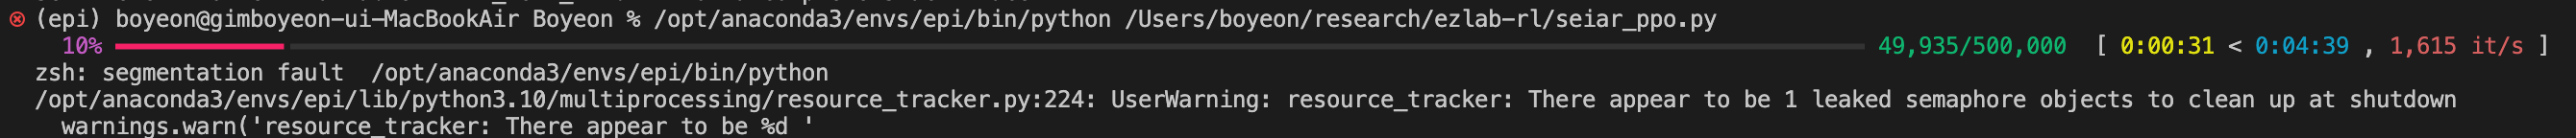
\includegraphics[width=15cm]{figures/error_m.png}
\end{frame}

\begin{frame}\frametitle{Next}
\begin{itemize}
    \item Google colab 연동(환경 맞추기)
    \item 500,000step까지 작동 확인
    \item Reward Design : Case1, Case2 Check!
\end{itemize}
\end{frame}

\end{document}